\documentclass{beamer}

%\documentclass[landscape,leqno]{beamer}
\usepackage{graphicx,color,amsmath,amssymb,amsfonts,amsbsy,amsthm,verbatim}
\usetheme{Berlin}
\newcommand{\includes}{/home/1104070/latex_include}
\newcommand{\dayonesegone}{day1_seg1_heuristic}
% Node the following tag will orient things right using dvi2pdf.
% Process with LaTeX first, then dvi2pdf.
\special{landscape}
\usepackage{float}
% Fuzz -----------------------------------------------------------
\hfuzz5pt % Don't bother to report overfull boxes < 5pt
% MATH -----------------------------------------------------------
\input{\includes/kalman_cmdmaster.tex}
% THEOREM ENV. ---------------------------------------------------
\newtheorem{thm}{Theorem.}
\newtheorem{cor}[thm]{Corollary.}
\newtheorem{con}[thm]{Conjecture.}
\newtheorem{lem}[thm]{Lemma.}
\newtheorem{prop}[thm]{Proposition.}
\newtheorem{defn}[thm]{Definition.}
\renewcommand{\thethm}{}  % unnumbered
\pagestyle{plain}
%%% --------------------------------------------------------------
\begin{document}
\title{
\vfill \hrulefill \vfill
\begin{center}
Basic Concepts of Navigation\\
\end{center}
}
\author{Michael L. Carroll}
\date{Sep 4, 2018\\
\vfill \hrulefill \vspace*{.25in} \vfill
\begin{tiny}
\copyright 2018
 by Michael L. Carroll
\end{tiny}
}
\maketitle

% ----------------------------------------------------------------
\begin{frame}
\frametitle{\textbf{Basic Concepts of Navigation\\Part I\\}}
 \begin{itemize}
 \item Overview
 \item The Navigation Problem and Reference Frames
 \item Inertial Navigation
\end{itemize}
\end{frame}
\begin{frame}
\frametitle{Overview}
\begin{itemize}
  \item Etymology of the term 'Navigation':  Latin $navis$='ship' and $agere$='to move or direct'
  \item Arose out of marine or ship navigation due to the challenge of navigating without landmarks
  \item Modern distinction between navigation and guidance
  \begin{itemize}
    \item navigation associated with state determination (open loop)
    \item guidance associated with control feedback (closed loop)
  \end{itemize} 
\end{itemize} 
\end{frame}

\begin{frame}
  \frametitle{The Navigation Problem from a Mathematical Perspective}
With respect to some mathematical reference frame, determine ...
\begin{itemize}
  \item vector displacement (3d position) and its time derivatives (velocity, acceleration, ...)
  \item rotational orientation (3d attitude) and its time derivatives (angular velocity, angular acceleration, ...) 
  \item Note:  This is a pure mathematics problem ... sensors do not enter into it
\end{itemize} 
\end{frame}


\begin{frame}
  \frametitle{The Navigation Problem from a Mathematical Perspective}
\begin{itemize}
  \item Reference frame is crucial:
  \begin{itemize}
    \item Position:  origin and three linearly independent vectors yields three numbers
    \item Attitude:  rotations about three linearly indepedent vectors yields three numbers
  \item I.e., 6 DOF = six degrees of freedom (3 position coordinates + 3 attitude coordinates)
  \end{itemize}
\end{itemize} 
\end{frame}


\begin{frame}
 \frametitle{The Navigation Problem from a Real World Physical Perspective}
\begin{itemize}
  \item Which reference frame should we use?
  \item Rectilinear or curvilenar coordinate system?
\end{itemize} 
\end{frame}

\begin{frame}
 \frametitle{The Navigation Problem from a Real World Physical Perspective}
\framesubtitle{Position}
For terrestrial navigation, global spherical (spheroidal) coordinates are used:
\begin{itemize}
  \item Latitude:  $\pm 90$ degrees north(+) or south(-) of the equator.
  \item Longitude: $\pm 180$ degrees east(+) or west(-) of the prime meridian through Greenwich, England
  \item Height:  Above the ellipsoid (normal to surface), or radius from center of earth
\end{itemize} 
\end{frame}

\begin{frame}
 \frametitle{The Navigation Problem from a Real World Physical Perspective}
\framesubtitle{Direction:  Bearing, Course, Track}
\begin{itemize}
  \item North Reference:  True and Magnetic. Direction angles are usually referenced clockwise with respect to north.
  \item  Bearing:  The angle with respect to north from one point on earth to another
  \item  Track:    The angle made by velocity vector with respect to north
  \item  Course:   Sometimes used synonym for track; sometimes expresses desired track vs. actual track
  \item  Heading:  Direction vehicle is pointing in with respect to north
\end{itemize} 
\end{frame}

\begin{frame}
 \frametitle{The Navigation Problem from a Real World Physical Perspective}
\framesubtitle{The Need for Sensors}
\begin{itemize}
  \item Reference frames are necessary, but not sufficient for real world navigation
  \item Also need real world sensor measurement data indicative of locations, distances, angles, etc. with respect to these reference frames
  \item But real world sensors are not perfect!  They only provide apparent positions, distances, angles, etc.
\end{itemize} 
\end{frame}

% day3_seg1_navproblem/navproblem_main.tex
\begin{frame}
\frametitle{\textbf{The Navigation Problem and Reference Frames}}
\framesubtitle{Topics}
 \begin{itemize}
 \item Basic Navigation Problem and Solutions
 \item Earth Referenced Navigation
 \item Coordinate Frame Conversion
 \item Basic Strapdown Navigation Equations
\end{itemize}
\end{frame}

% day3_seg1_navproblem/basicnavprob.tex
%\begin{frame}
%Solutions to the Basic Navigation Problem\\
%Solution in Inertial Space
% \begin{itemize}
% \item In an inertial reference frame, it's no problem, if you 
% have a cluster of inertial sensors and you know your initial 
% position:
% \item Just integrate the acceleration once to get velocity, 
%twice to get
% position.
%\[v(T) = v(0) + \int_{0}^{T}\dfrac{d^2r}{dt^2}dt\]
%\[r(T) = r(0) + \int_{0}^{T}v(t)dt\]
% \item And integrate the angular rate once to get attitude.
%\end{itemize}
%\end{frame}

%\begin{frame}
%Solution in Inertial Space
%\begin{itemize}
%  \item Solution easy in inertial space because ...
%  \begin{itemize}
%	\item inertial instruments sense acceleration and rotational % rate with respect to inertial coordinate frame 
%	\item inertial frame attached to sensor platform
%    \item Note: You still need to rotate accelerations from body %to inertial coordinates prior to integration (strapdown)
%  \end{itemize}
%  \item But we don't necessarily want the answer to our 
%questions expressed in terms of inertial coordinates!
%\end{itemize} 
%\end{frame}

\begin{frame}
\frametitle{Dead Reckoning}
\begin{itemize}
  \item Process of determining new position based on extrapolating from previously known position and velocity.
  \item Velocity = Speed and Direction
  \item Unaided inertial navigator is essentially a dead reckoning computer
\end{itemize} 
\end{frame}






% day3_seg1_navproblem/earthrev.tex
\begin{frame}
\frametitle{Earth Referenced Navigation}
 \begin{itemize}
 \item Terrestial navigation seeks to answer nav questions with respect to earth
 \begin{itemize}
   \item Global earth reference
   \item Local or relative navigation
 \end{itemize}
 \item Complications:
 \begin{itemize}
   \item Earth surface is curved (ellipsoid)
   \item Earth is turning (can usually ignore motion about the Sun for terrestrial nav)
 \end{itemize}
\end{itemize}
\end{frame}

\begin{frame}
\frametitle{Earth Model:  WGS 84}
\begin{itemize}
  \item Earth is not spherical, but oblate spheroid or ellipsoid
  \item Flattened at the poles
  \item World Geodetic System 84:
  \begin{itemize}
   \item Semi-major axis:  6,378,137.0 m
        \item Semi-minor axis:  6,356,752.314  m
  \end{itemize}
  \item Not the same as geoid:  no terrain or gravity model
\end{itemize} 
\end{frame}

% day3_seg1_navproblem/coordconv.tex
\begin{frame}
\frametitle{Coordinate Frames}
 \begin{itemize}
 \item Inertial
 \item Earth Fixed
 \item Local Level
 \item Body
\end{itemize}
\end{frame}
\begin{frame}
\frametitle{Coordinate Frames}
 \begin{itemize}
  \item Technically speaking, all frames are earth-centered
  \begin{itemize}
    \item Common origen needed for linear transformations (such as rotations)
    \item Can compensate by using a translation
  \end{itemize}
  \item Practically speaking, we think of the Body frame as centered in the body of the vehicle (usually at center of gravity).
  \item Local Level is thought to be located at surface of earth directly beneath the vehicle.
\end{itemize}
\end{frame}
\begin{frame}
\frametitle{Inertial Reference Frames}
 \begin{itemize}
 \item Non-Rotating
 \item Non-Accelerating
 \item Fixed or moving uniformly with respect to another inertial
 frame (fixed stars)
\end{itemize}
\end{frame}

\begin{frame}
\frametitle{Inertial Reference Frames}
 \begin{itemize}
 \item Nav problem "easy" in inertial frames
 \item Integrate gyro rates once to get attitude (rotational motion independent of lateral motion)
 \item Rotate accelerometer outputs to inertial frame using attitude matrix, then integrate to get inertial
 velocity; integrate velocity to get position.
 \item Would still have to contend with instrument imperfections.
\end{itemize}
\end{frame}

\begin{frame}
\frametitle{Inertial Reference Frame Integrations}
\begin{equation}\label{inertacceleq}
\ddot{r}(t)=\specforce+\text{other external forces}
\end{equation}
\begin{equation}\label{inertveleq}
v(T)=\dot{r}(T)=v(0)+\int_{0}^{T}\specforce dt + \int_{0}^{T}(\text{other
external forces})dt
\end{equation}
\begin{equation}\label{inertposeq}
  r(T)=r(0)+\int_{0}^{T}v(t)dt
\end{equation}
\end{frame}

\begin{frame}
\frametitle{Earth Fixed = ECEF = Earth Centered Earth Fixed}
 \begin{itemize}
 \item Rotating frame, i.e., non-inertial
 \item Cartesian ($X,Y,Z$ in meters)
 \item Spherical (latitude $\lat$, longitude $\lon$, altitude $\alt$)
 \begin{itemize}
 \item geodetic
 \end{itemize}
\end{itemize}
\end{frame}


\begin{frame}
\frametitle{Local Level}
 \begin{itemize}
 \item Tangent to earth's surface but translated to center of
 earth.
 \item Vertical $Z$-axis is normal to earth's surface
 \item $X,Y$-axes are level
 \item Several kinds: $Y$ north-slaved, wander (0 transport rate) or free azimuth
 \item $Y$ makes wander angle $\alpha$ with respect to true north (ENU=East, North, Up).
\end{itemize}
\end{frame}

\begin{frame}
\frametitle{Earth Centered, Earth Fixed:  ECEF}
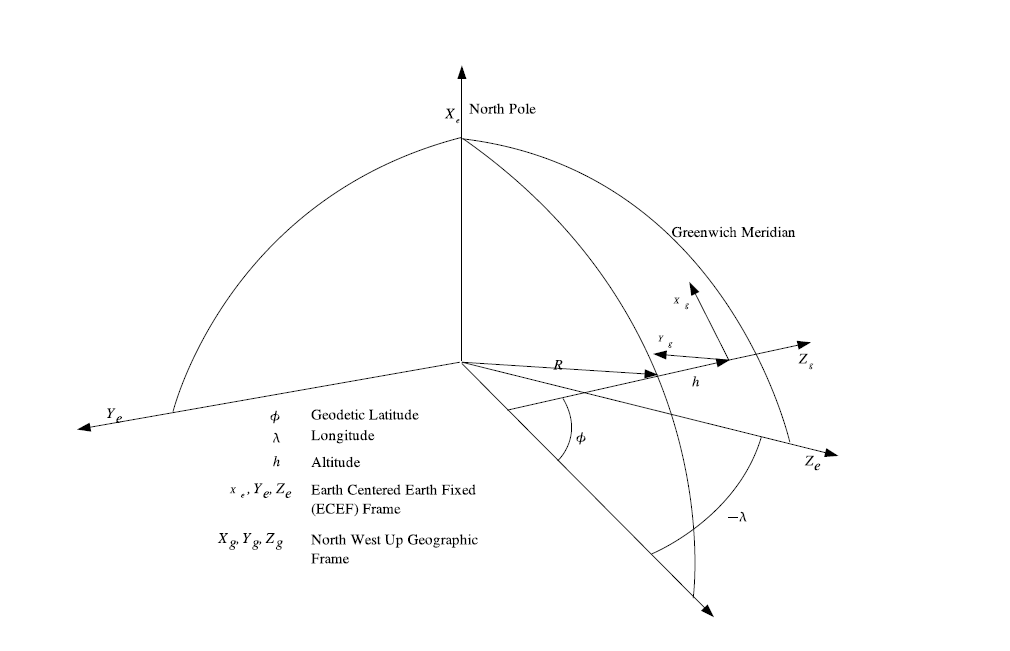
\includegraphics[width=\textwidth]{graphics/ecef.png}
\vfill
\end{frame}


\begin{frame}
\frametitle{Body Frame}
 \begin{itemize}
 \item Attached to vehicle
 \item For aircraft:
   \begin{itemize}
    \item $X$ out the nose
    \item $Y$ out the right wing
    \item $Z$ down
   \end{itemize}
\end{itemize}
\end{frame}

\begin{frame}
\frametitle{Body Frame (cont)}
 \begin{itemize}
 \item For space vehicles RIC:
   \begin{itemize}
    \item $R$ downward on radius to center of earth
    \item $I$ in-track, in direction of motion
    \item $C$ cross-track, perpendicular to motion
   \end{itemize}
 \item Also sometimes referred as RAC, where 'A' stands for 'along-track'
\end{itemize}
\end{frame}

\begin{frame}
\frametitle{Coordinate Frame Conversion}
 \begin{itemize}
 \item All frames earth-centered, differing only by
 rotation
 \item Rotation represented by direction cosine matrix (DCM) or set of four quaternions
 \begin{itemize}
	\item Expresses angles made by basis vectors of one frame with those of another
 \end{itemize}
 \item $\dcm{A}{B}$ = DCM transformation from frame A to frame B
\end{itemize}
\end{frame}

\begin{frame}
\frametitle{Coordinate Frame Conversion}
\begin{itemize}
  \item "Direction Cosine" comes from dot product:
\[\ip{x}{y}=x\cdot y=\norm{x}\norm{y}\cos\theta_{xy}\]
where $\theta_{xy}$ is the angle between the two vectors $x$ and $y$.
  \item If $x$ and $y$ are unit vectors, then $\norm{x}=\norm{y}=1$ and we have:
\[\ip{x}{y}=x\cdot y=\cos\theta_{xy}\]
\end{itemize} 
\end{frame}

\begin{frame}
\frametitle{Coordinate Frame Conversion}
\begin{itemize}
  \item If $U=\set{u_1,u_2,u_3}$ and $V=\set{v_1,v_2,v_3}$ are two sets of orthonormal basis vectors, then the DCM relating one frame to the other is given by:
\begin{align*}
\dcm{U}{V}&=
\begin{bmatrix}
\ip{u_1}{v_1} & \ip{u_1}{v_2} & \ip{u_1}{v_3}\\
\ip{u_2}{v_1} & \ip{u_2}{v_1} & \ip{u_2}{v_3}\\
\ip{u_3}{v_1} & \ip{u_3}{v_2} & \ip{u_3}{v_3}\\
\end{bmatrix}\\
&=
\begin{bmatrix}
\cos\theta_{11} & \cos\theta_{12} & \cos\theta_{13}\\
\cos\theta_{21} & \cos\theta_{22} & \cos\theta_{23}\\
\cos\theta_{31} & \cos\theta_{32} & \cos\theta_{33}\\
\end{bmatrix}
\end{align*}
\end{itemize} 
\end{frame}

\begin{frame}
\frametitle{Coordinate Frame Conversion}
\begin{itemize}
  \item If $V=\set{v_1,v_2,v_3}$ is considered to be the reference frame and its units vectors are the standard basis so that 
\[
v_1=\begin{bmatrix}
	1\\
	0\\
	0\\
	\end{bmatrix},
v_2=\begin{bmatrix}
	0\\
	1\\
	0\\
	\end{bmatrix},
v_3=\begin{bmatrix}
	0\\
	0\\
	1\\
	\end{bmatrix},
\]
then the DCM simplifies to just the coordinates of $u_1,u_2,u_3$ vectors with respect to $V$:
\begin{align*}
\dcm{U}{V}&=
\begin{bmatrix}
u_{11}& u_{12} & u_{13}\\
u_{21} & u_{22} & u_{23}\\
u_{31} & u_{32} & u_{33}\\
\end{bmatrix}
\end{align*}
\end{itemize} 
\end{frame}


\begin{frame}
\frametitle{Coordinate Frame Conversion}
 \begin{itemize}
 \item DCMs are (real) orthogonal matrices $\Rightarrow \left[\dcm{A}{B} \right]^{-1}=\left[\dcm{A}{B} \right]\trans=\dcm{B}{A}$
 \item Third row (or column) is vector cross product of other two\\
 $\Rightarrow$ only six independent parameters
 \item DCMs satisfy:   $\dcm{B}{A}\dcm{C}{B}=\dcm{C}{A}$
\end{itemize}
\end{frame}

\begin{frame}
\frametitle{Coordinate Frame Conversion}
 \begin{itemize}
 \item Orthogonal matrices preserve lengths of vectors: $\norm{Rx}=\norm{x}$
 \item Orthogonal matrices also preserve angles between vectors:  $\ip{Rx}{Ry}=\ip{R\trans Rx}{y}=\ip{Ix}{y}=\ip{x}{y}$
 \item Intuitively obvious in the case of rotations
\end{itemize}
\end{frame}

\begin{frame}
\frametitle{DCMs and Euler Rotation}
 \begin{itemize}
 \item Euler showed that three simultaneous rotations about three orthogonal axes can be
viewed as a single rotation about a single axis
 \item The single angle $\theta$ of rotation for a DCM can be determined from the eigenvalues of the DCM, which are:
\[
\set{1, \exp(i\theta), \exp(-i\theta)}
\]
\item The determinant of a DCM is therefore always 1.   Why? (Hint: How do you compute the determinant from the eigenvalues?)
\end{itemize}
\end{frame}

\begin{frame}
\frametitle{Euler Rotation}
\begin{figure}[h]
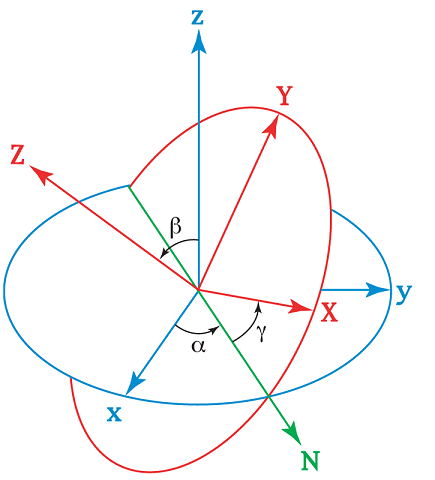
\includegraphics[width=0.5\textwidth]{graphics/euler.png}
\end{figure}
\end{frame}


\begin{frame}
\frametitle{DCMs and Euler Rotation}
 \begin{itemize}
 \item The axis of rotation for the single Euler rotation can be found from DCM as follows:
\begin{align*}
\dcm{U}{V}&=
\begin{bmatrix}
u_{11}& u_{12} & u_{13}\\
u_{21} & u_{22} & u_{23}\\
u_{31} & u_{32} & u_{33}\\
\end{bmatrix}
\end{align*}
then the axis of rotation $r = [r_1,r_2,r_3]\trans$ is given by
\begin{align*}
r_1 &= u_{12}u_{23} - (u_{22}-1)u_{13}\\
r_2 &= u_{21}u_{13} - (u_{11}-1)u_{23}\\
r_3 &= (u_{11}-1)(u_{22}-1) - u_{12}u_{21}\\
\end{align*}
\end{itemize}
\end{frame}

\begin{frame}
\frametitle{DCMs and Quaternions}
 \begin{itemize}
 \item If $C$ is a direction cosine matrix with elements $c_{ij}$, then the following four quantities define a quaternion of the rotation:
\begin{align*}
q_1 &= \dfrac{1}{4q_4}(c_{23}-c_{32})\\
q_2 &= \dfrac{1}{4q_4}(c_{13}-c_{31})\\
q_3 &= \dfrac{1}{4q_4}(c_{21}-c_{12})\\
q_4 &= \pm \dfrac{1}{2}\sqrt{1+c_{11}+c_{22}+c_{33}}\\
\end{align*}
\end{itemize}
\end{frame}

\begin{frame}
\frametitle{DCMs and Quaternions}
 \begin{itemize}
 \item It's even simpler to obtain quaternions from Euler rotation angle $\theta$ and axis given by a unit vector $u$:
\[q_i=u_i\sin(\theta/2), \text{ for } i=1,2,3\]
and
\[q_4=\cos(\theta/2)\]
\end{itemize}
\end{frame}


\begin{frame}
\frametitle{Coordinate Frame Conversion: Most important DCMs for terrestrial navigation}
 \begin{itemize}
 \item Body to Local Level: $\dcm{B}{L}$
 \begin{itemize}
 \item sometimes called Body to Nav and notated $\dcm{B}{N}$
 \item yields attitude info (Euler angles for roll, pitch, yaw)
 \end{itemize}
 \item Local Level to Earth: $\dcm{L}{E}$
 \begin{itemize}
 \item yields position info and also used to transform earth rate to
 local level
 \end{itemize}
\end{itemize}
\end{frame}
\begin{frame}
\frametitle{Coordinate Frame Conversion: Most important DCMs}
\begin{itemize}
  \item Visualize $\dcm{L}{E}$'s determination of position as follows:
	\begin{itemize}
		\item As vehicle moves, local level frame changes its orienation with respect to earth's center in order to maintain local level with respect to earth's surface
		\item If you think of local level frame as attached to earth's surface, you get distracted by the displacement of the frame
		\item If you move local level frame to center of earth, the displacement disappears and all that remains are the rotations
	\end{itemize} 
\end{itemize} 
\end{frame}

\begin{frame}
\begin{figure}
\centering
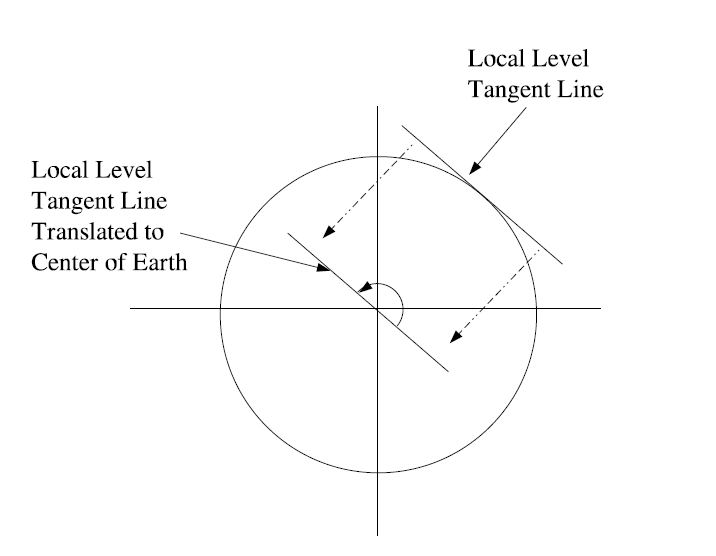
\includegraphics[width=\textwidth]{graphics/local_level.png}
\caption{Local Level to Earth Transformation}
\end{figure}
\end{frame}
% day3_seg1_navproblem/strapdown.tex
\begin{frame}
\frametitle{Inertial navigation Systems}
\framesubtitle{Strapdown Navigation:  Strapdown vs. Gimbaled}
\begin{itemize}
  \item Gimbaled INS:
  \begin{itemize}
	\item Gyro stabilized platform
	\item Gimbal assembly and torque motors
	\item Resolvers, slip rings, bearings, etc. to control  platform
	\item Goal: Maintain stable, locally level or inertial reference frame
  \end{itemize}
\end{itemize} 
\end{frame}


\begin{frame}
\frametitle{Strapdown Navigation: Strapdown vs. Gimbaled}
\begin{itemize}
  \item Gimbaled INS Issues
  \begin{itemize}
	\item Reliability and Cost: Lots of moving parts!
	\item Body rate and acceleration information not directly available
	\item Rate signals are generally noisy and have low bandwidth
  \end{itemize}
\end{itemize} 
\end{frame}


\begin{frame}
\frametitle{Strapdown Navigation: Strapdown vs. Gimbaled}
\begin{itemize}
  \item Strapdown INS:
  \begin{itemize}
	\item Inertial instruments strapped to body frame
	\item Requires local level accelerations to be computed using direction cosine matrix $\dcm{B}{L}$
	\item $\dcm{B}{L}$ derived from gyro-sensed body rates
    \item Strapdown systems can be implemented with either rate gyros or attitude gyros 
  \end{itemize} 
\end{itemize} 
\end{frame}

\begin{frame}
\frametitle{Strapdown Navigation: Strapdown vs. Gimbaled}
\begin{itemize}
  \item Strapdown INS Advantages
  \begin{itemize}
	\item Immediate detection of body rates and accelerations
	\item Fewer moving parts
	\item Potential redundancy advantages
  \end{itemize} 
  \item Gimbaled systems are nearly obsolete
\end{itemize} 
\end{frame}

\begin{frame}
\frametitle{Strapdown Inertial Block Diagram}
\begin{center}
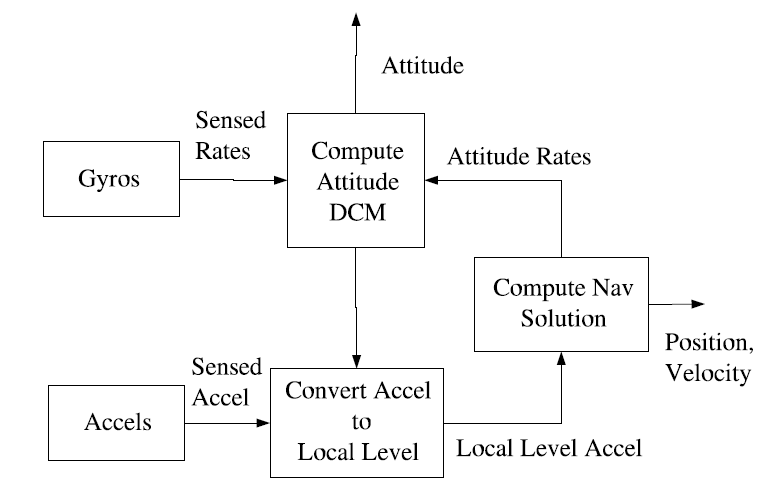
\includegraphics[scale=0.5]{graphics/strapdown_block.png}
\end{center}
\end{frame}

\begin{frame}
\frametitle{Basic Strapdown Navigation Equations}
 \begin{itemize}
 \item Need to compute attitude, velocity, and position
 \item I.e., need to compute $\dcm{B}{L}$ and $\dcm{L}{E}$
 \item These DCMs are dynamic quantities
 \item $\dcm{B}{L}$ determines attitude and can be rapidly varying
 \item $\dcm{L}{E}$ determines position and is slowly varying (relative to attitude dynamics)
\end{itemize}
\end{frame}


\begin{frame}
\frametitle{Strapdown Navigation Equations}
 \begin{itemize}
 \item Three differential equations
 \begin{itemize}
   \item Equation for body to local level transformation $\dcm{B}{L}$
   \item Equation for velocity (uses $\dcm{B}{L}$)
   \item Equation for local level to earth for position DCM $\dcm{L}{E}$
 \end{itemize}
\end{itemize}
\end{frame}

\begin{frame}
Strapdown Navigation Equations
 \begin{itemize}
 \item Two Algebraic Equations
 \begin{itemize}
   \item Equation for converting velocity to transport rate (to be explained)
   \item Equation for converting earth rate to local level
   coordinates
 \end{itemize}
\end{itemize}
\end{frame}
\begin{frame}
\frametitle{Strapdown Navigation Equations}
\framesubtitle{The Three Differential Equations}
\begin{equation}\label{cbleq}
  \cbleq
\end{equation}
\begin{equation}\label{strapveleq}
  \strapveleq
\end{equation}
\begin{equation}\label{cleeq}
  \cleeq
\end{equation}
\end{frame}

\begin{frame}
\frametitle{Strapdown Navigation Equations}
\framesubtitle{The Two Algebraic Equations}
\begin{equation}\label{trateeq}
  \trateeq \text{ (wander azimuth $\rho_z=0$)}
\end{equation}
\begin{equation}\label{erateeq}
  \erateeq
\end{equation}
\end{frame}

\begin{frame}
\frametitle{Strapdown Navigation Equations}
The $\dcm{B}{L}$ Equation \eqref{cbleq}
\[\cbleq\]
\begin{itemize}
\item All the $\Omega$ matrices represent rotation vector cross products in skew-symmetric matrix format
\begin{itemize}
 \item $\rotmat{I}{B}^B$ is rotational rate of aircraft in body
coordinates
\item $\rotmat{I}{E}^L$ is earth rate in local level coordinates
\item $\rotmat{E}{L}^L$ is transport rate in local level
coordinates
\end{itemize}
\end{itemize}
\end{frame}

\begin{frame}
\frametitle{Strapdown Navigation Equations: Detour into Cross Product Matrices}
\begin{itemize}
\item The cross product of $\omega=\colvecthree{\omega}{}$ with any other vector $v$ is the same as multiplying $v$ on the left by
$\Omega = \skewsymmat{\omega}{1}{2}{3}$
\item $\omega \times v=\Omega v$
\end{itemize}
\end{frame}

\begin{frame}
\frametitle{Strapdown Navigation Equations}
The $\dcm{B}{L}$ Equation \eqref{cbleq}
\[\cbleq\]
\begin{itemize}
\item Transport rate is the rotational rate of the aircraft due to
motion over the surface of the earth.  Is a function of velocity.
\item $\rotmat{I}{B}^B$ is total inertial angular rate sensed by gyros and includes effects of
transport and earth rates.
\item Hence transport and earth rate effects have to be subtracted
off.
\end{itemize}
\end{frame}

\begin{frame}
\frametitle{Strapdown Navigation Equations}
\framesubtitle{The Strapdown Velocity Equation} \eqref{strapveleq}
\[\strapveleq\]
 \begin{itemize}
 \item Sometimes referred to as the velocity rate equation
 \item $\specforce^B$ is specific force sensed by accelerometers in
 body coordinates (because the accels are strapped to the body --
 hence the term strapdown)
\end{itemize}
\end{frame}

%\begin{frame}
%\includegraphics[width=10in,height=6.5in]{strapnav_block.png}
%\end{frame}

\begin{frame}
\frametitle{Strapdown Navigation Equations}
\framesubtitle{The Transport Rate Equation}
 \eqref{cleeq}
\[\cleeq\]
\begin{itemize}
  \item Connected to velocity rate equation by the first algebraic equation \eqref{trateeq}:
\[\trateeq\]
  \item Eq. \eqref{cleeq} Sometimes referred to as position rate equation, because $\dcm{L}{E}$ directly implies the vehicle position
\end{itemize} 
\end{frame}

\begin{frame}
\frametitle{Strapdown Navigation Equations}
\framesubtitle{Position Rate / Transport Rate Equations (Geographic)}
\begin{itemize}
  \item North transport rate:
\begin{equation}\label{trateneq}
\trateneq
\end{equation} 
  \item East transport rate:
\begin{equation}\label{trateeeq}
\trateeeq
\end{equation} 
where $e$ is ellipticity (approx. $\dfrac{1}{298}$) and $R_e$ is mean equatorial earth radius
\end{itemize} 
\end{frame}

\begin{frame}
\frametitle{Strapdown Navigation Equations}
\framesubtitle{Position Rate / Transport Rate Equations (Geographic)}
\begin{itemize}
  \item Latitude Rate:
\begin{equation}\label{latrate}
\latrateeq
\end{equation}  
  \item Longitude Rate:
\begin{equation}\label{lonrate}
\lonrateeq
\end{equation}  
\end{itemize} 
\end{frame}

\begin{frame}
\frametitle{Strapdown Navigation Equations}
\begin{itemize}
  \item Geographic (north-slaved) mechanization has singularities at poles
  \item Two other approaches to local level coordinates:
  \begin{itemize}
	\item Free azimuth: vertical component of transport rate $\rho_z$= additive inverse of vertical component of earth rate
	\item Wander Azimuth:  vertical component of transport rate $\rho_z$ = 0
  \end{itemize}
\end{itemize} 
\end{frame}

\begin{frame}
\frametitle{Strapdown Navigation Equations}
\framesubtitle{Position Rate / Transport Rate Equations (Wander and Free Azimuth)}
\begin{itemize}
  \item X Transport Rate:
\begin{align}\label{xtrateeq}
\xtrateeq
\end{align}  
  \item Y Transport Rate:
\begin{align}\label{ytrateeq}
\ytrateeq
\end{align}  
\end{itemize} 
\end{frame}

\begin{frame}
\frametitle{Strapdown Navigation Equations}
\framesubtitle{Position Rate / Transport Rate Equations (Wander and Free Azimuth)}
\begin{itemize}
  \item Azimuth Rate:
\[
\rho_z= 
\begin{cases} 
-\erate d_{23}, &\text{if free azimuth;}\\ 
0,  &\text{if wander azimuth} 
\end{cases}
\]
  \item In equations above, the matrix $\left[d_{ij}\right]$ is the direction cosine matrix $\dcm{L}{E}$ from local level (L) frame to earth centered earth fixed (E) frame.
\end{itemize} 
\end{frame}


\begin{frame}
\frametitle{GPS}
\begin{itemize}
  \item Trilateration:  Knowing the distance from an unknown point to three known points yields the coordinates of the unknown point
  \item What if the distances are not known precisely?  
Answer:  Use 'pseudorange' instead, i.e., use signals traveling at speed of light and very accurate clocks
  \item What if the coordinates of the three points are not really known precisely?  Answer:  Use your best guess!
\end{itemize} 
\end{frame}

\begin{frame}
	\frametitle{Trilateration}
	\begin{figure}
	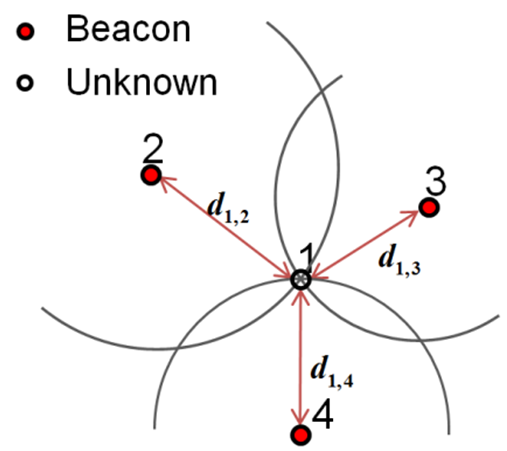
\includegraphics[width=0.5\textwidth]{graphics/trilateration.png}
\caption{Trilateration:  Distances to Three Beacons}
	\end{figure}
\end{frame}


\begin{frame}
	\frametitle{Pseudorange}
	\begin{itemize}
		\item distance = (speed of signal) $\times$ (time of signal flight)
		\begin{itemize}
			\item $\rho = c\Delta t$
		\end{itemize}
		\item Called 'pseudorange' because it is not a true range; it is only apparent due to inaccurate clocks
		\item By the same token, the coordinates of the transmitting satellites are also not known precisely, and so we could speak of 'pseudopositions' as well.   But nobody does that!
	\end{itemize}
\end{frame}

\begin{frame}
	\frametitle{Satellite Position}
	\begin{itemize}
		\item How do we know which satellite is transmitting? Answer:  Unique Pseudorandom Noise (PRN)
		\item How we know the position of the 
satellite at time of transmission?  Answer:
		\begin{itemize}
			\item Six Keplerian elements
			\item User receiver converts to WGS-84 X,Y,Z ECEF coordinates
		\end{itemize}
	\end{itemize}
\end{frame}

\begin{frame}
	\frametitle{Six Keplerian Elements}
	\begin{itemize}
		\item Eccentricity
		\item Semi-major axis
		\item Inclination
		\item Longitude of the ascending node
		\item Argument of periaspsis
		\item Mean anomaly
	\end{itemize}
\end{frame}

\begin{frame}
\frametitle{Keplerian Elements}
	\begin{figure}
	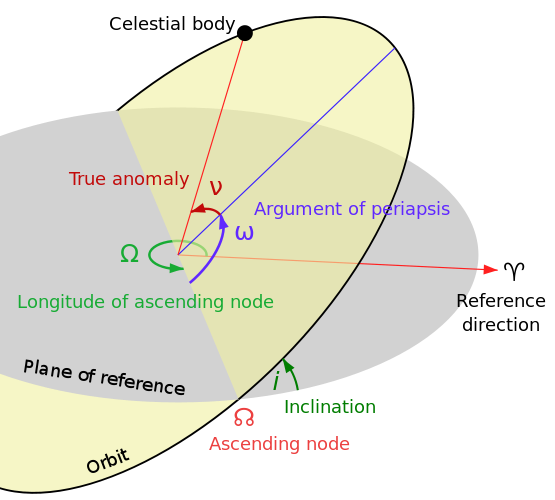
\includegraphics[width=0.75\textwidth,height=0.75\textheight]{graphics/555px-Orbit1_svg.png}
%	\caption{Keplerian Elements}
	\end{figure}
\end{frame}

\begin{frame}
\frametitle{Keplerian Elements}
	\begin{figure}
	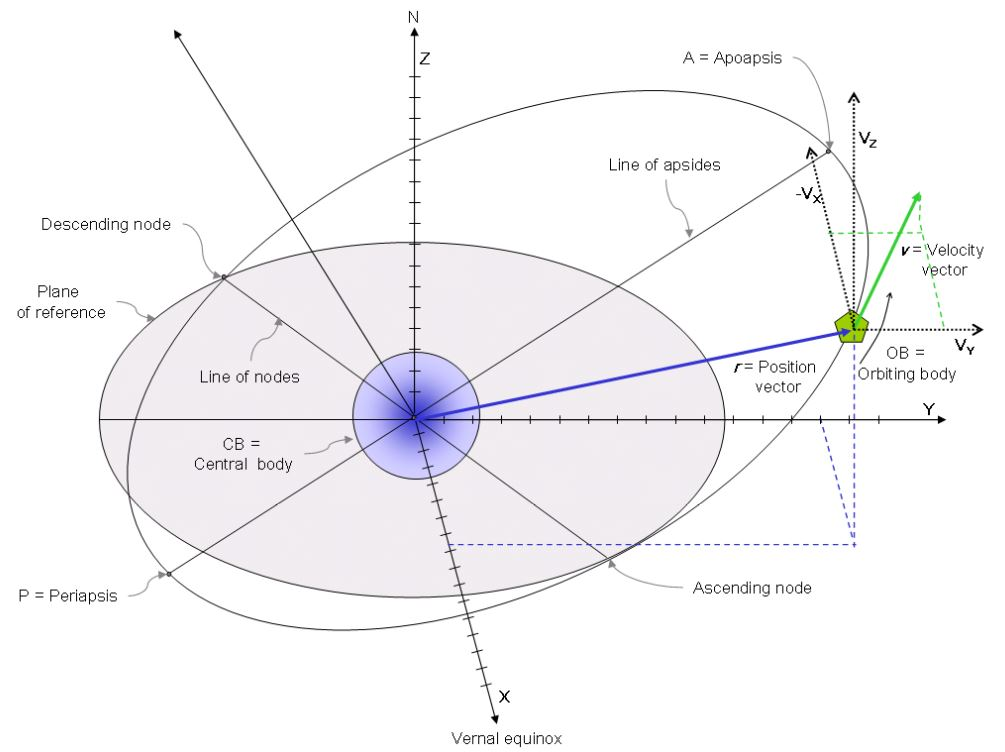
\includegraphics[width=0.80\textwidth,height=0.80\textheight]{graphics/keplerian_elements2.jpg}
%	\caption{Keplerian Elements}
	\end{figure}
\end{frame}

\begin{frame}
\frametitle{IS-GPS-200 Table 20-II}
\framesubtitle{1 of 2}
	\begin{figure}[h]
	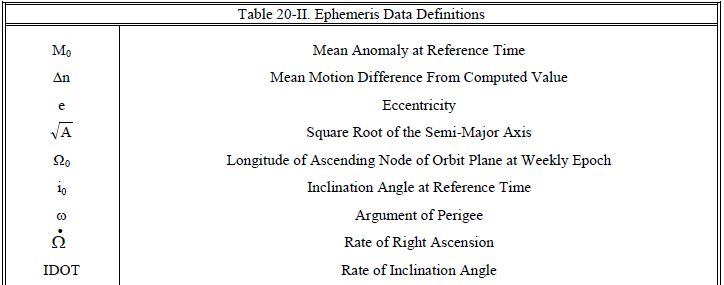
\includegraphics[width=0.8\textwidth]{graphics/table20-II-A.jpg}
%	\caption{Keplerian Elements}
	\end{figure}
\end{frame}

\begin{frame}
\frametitle{IS-GPS-200 Table 20-II}
\framesubtitle{2 of 2}
	\begin{figure}[h]
	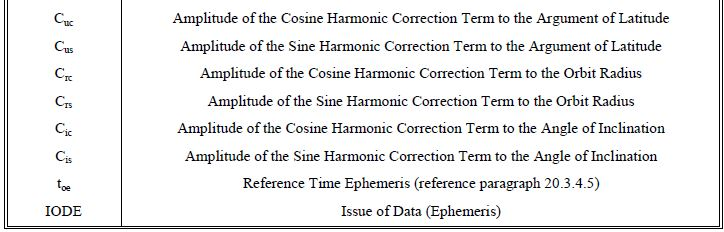
\includegraphics[width=0.8\textwidth]{graphics/table20-II-B.jpg}
%	\caption{Keplerian Elements}
	\end{figure}
\end{frame}

\begin{frame}
\frametitle{IS-GPS-200 Table 20-IV}
\framesubtitle{Elements of Coordinate Systems (1 of 3)}
	\begin{figure}[h]
	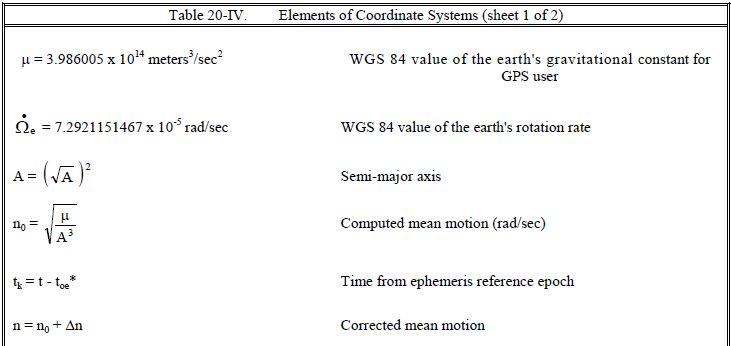
\includegraphics[width=0.8\textwidth]{graphics/table20-IV-A.jpg}
%	\caption{Keplerian Elements}
	\end{figure}
\end{frame}

\begin{frame}
\frametitle{IS-GPS-200 Table 20-IV}
\framesubtitle{Elements of Coordinate Systems (2 of 3)}
	\begin{figure}[h]
	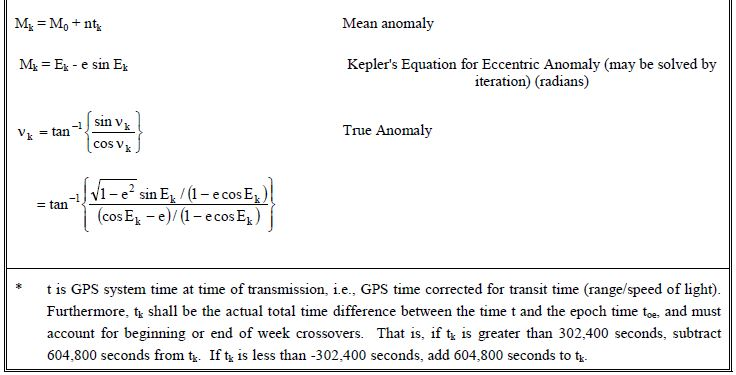
\includegraphics[width=0.8\textwidth]{graphics/table20-IV-B.jpg}
%	\caption{Keplerian Elements}
	\end{figure}
\end{frame}

\begin{frame}
\frametitle{IS-GPS-200 Table 20-IV}
\framesubtitle{Elements of Coordinate Systems (3 of 3)}
	\begin{figure}[h]
	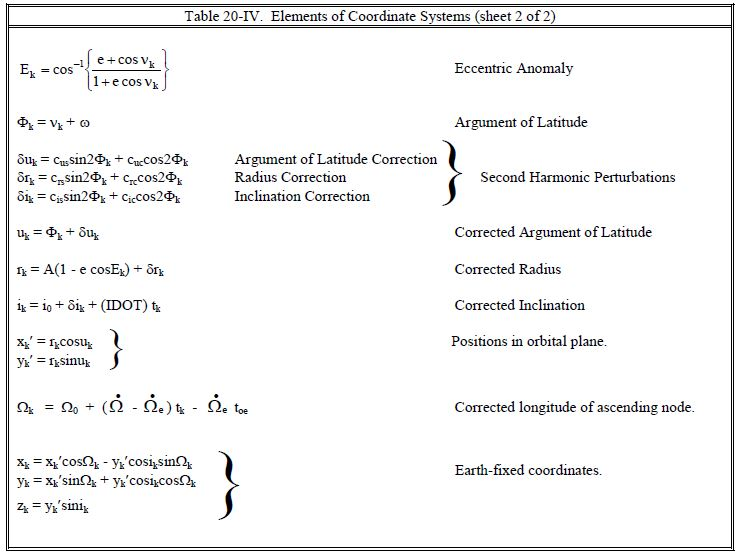
\includegraphics[width=0.8\textwidth]{graphics/table20-IV-C.jpg}
%	\caption{Keplerian Elements}
	\end{figure}
\end{frame}


% ----------------------------------------------------------------
\end{document}
